\chapter{Implementation}
\label{chap3}

\section{Triangulation of regular implicit srufaces}
\label{triangulation-implicit}

In this section, we shortly describe the algorithm for triangulation of the regular
parts of implicit surfaces introduced in bachelor's thesis \cite{korecova2021triangulation}.

The algorithm creates triangles iteratively, one at a time. The new triangle is
created at the edge of the existing triangle. The new point is projected on the
surface using the Newton-Rhapson method. This method finds the root of the implicit
function lying on the line, which is in the direction of the gradient of the implicit
function. This approach is displayed on the Figure \ref{img:29}.
\begin{figure}
    \centerline{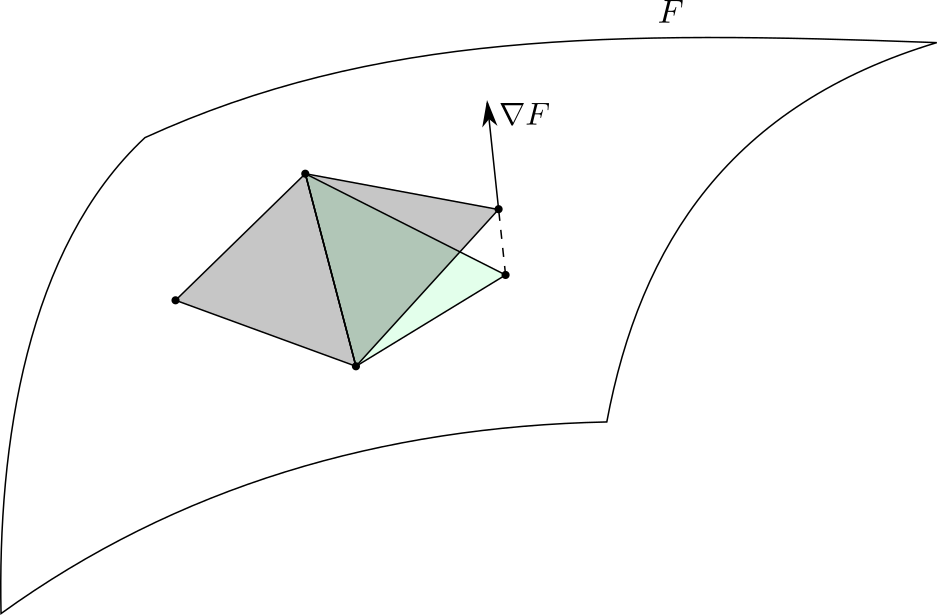
\includegraphics[scale=0.5]{images/img29}}
    \caption[TODO]
    {TODO}
    %id obrazku, pomocou ktoreho sa budeme na obrazok odvolavat
    \label{img:29}
\end{figure}

After the new point is projected on the surface, conditions are checked. 
Some of these conditions are based on the Delaunay triangulation introduced
by Hilton \cite{hilton1996marching}. The Delaunay condition checks,
if some other points are in the proximity of circumcenter of the new triangle.
The conditions minimize the chances of triangle intersection.
If the new triangle intersects with some existing triangles, the algorithm
tries to connect the new triangle to the existing triangles in its proximity.

The algorithm is enriched with the possibility to triangulate adaptively
to the curvature of the surface using approach presented by Akkouche 
\cite{akkouche2001adaptive}. It can also triangulate surfaces in the
bounded volume - axis aligned bounding box, given by six numbers - minimal
and maximal value for each of the three axes.

As a part of our work, we reimplement the algorithm to be more effective by
using advanced data structures, such as the half-edge data structure 
\cite{kettner1999using} and the range tree \cite{lueker1978data}. 
\section{Data structures for triangulation algorithm}
\label{sub2.5}

\subsection{Half-edge data structure}
Triangular mesh is given by a set of vertices, non-oriented edges and triangular faces.
There are multiple methods for mesh representation. The straightforward one -
list of vertices, edges and vertices does not provide any information about
the local surroundings of the vertices, edges and faces and therefore the searching
for incident faces or incident edges is complicated and inefficient.

In 1975, Baumgart \cite{baumgart1975polyhedron} presented a representation
using winged edges, which was further improved in 1985 by Weiler \cite{weiler1985edge}
who presented the modification called half-edge data structure.
Both of these representations are edge-based representations, each edge stores
references (pointers) to the surrounding vertices, edges and faces. One can easily extract the information of the
surrounding vertices, edges and faces.

In the winged edge representation, each edge is represented as oriented line segment 
and stores references to its vertices, both incident faces, left and right traverse. 
Each vertex stores a reference to one of the outgoing edges and each
face stores a reference to one of its incident edge. An example of such representation
is shown on the Figure \ref{img:30} and tables \ref{tab:2}, \ref{tab:3}, \ref{tab:4}.

\begin{figure}
    \centerline{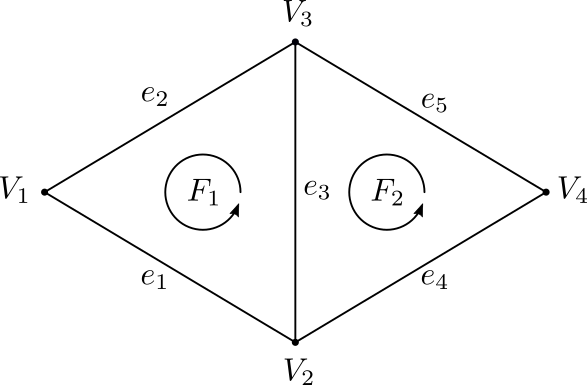
\includegraphics[scale=0.5]{images/img30}}
    \caption[Example of winged edge representation]
    {Example of winged edge representation.}
    %id obrazku, pomocou ktoreho sa budeme na obrazok odvolavat
    \label{img:30}
\end{figure}

\begin{table}[]\centering
    \begin{tabular}{|c|cc|cc|cc|cc|}
    \hline
    \hline
    Edge  & \multicolumn{2}{c|}{Vertex} & \multicolumn{2}{c|}{Face} & \multicolumn{2}{c|}{Left traverse} & \multicolumn{2}{c|}{Right traverse} \\ \hline
          & Initial      & Terminal     & Left        & Right       & Pred.            & Succ.           & Pred.            & Succ.            \\ \hline\hline
    $e_1$ & $V_1$        & $V_2$        & $F_1$       &             & $e_2$            & $e_3$           &                  &                  \\ \hline
    $e_2$ & $V_3$        & $V_1$        & $F_1$       &             & $e_3$            & $e_1$           &                  &                  \\ \hline
    $e_3$ & $V_2$        & $V_3$        & $F_1$       & $F_2$       & $e_1$            & $e_2$           & $e_5$            & $e_4$            \\ \hline
    $e_4$ & $V_2$        & $V_4$        & $F_2$       &             & $e_3$            & $e_5$           &                  &                  \\ \hline
    $e_5$ & $V_4$        & $V_3$        & $F_2$       &             & $e_4$            & $e_3$           &                  &                  \\ \hline\hline
    \end{tabular}
\caption{Edge table of a winged edge data structure for the Figure \ref{img:30}.}
\label{tab:2}
\end{table}

\begin{table}[]
    \centering
    \begin{tabular}{|c|ccc|c|}
    \hline
    \hline
    Vertex  & \multicolumn{3}{c|}{Coordinates}          & Edge            \\ \hline
          & x            & y            & z           & Outgoing edge   \\ \hline\hline
    $V_1$ & $x_1$        & $y_1$        & $z_1$       & $e_1$           \\ \hline
    $V_2$ & $x_2$        & $y_2$        & $z_2$       & $e_4$           \\ \hline
    $V_3$ & $x_3$        & $y_3$        & $z_3$       & $e_2$           \\ \hline
    $V_4$ & $x_4$        & $y_4$        & $z_4$       & $e_5$           \\ \hline\hline
    \end{tabular}
\caption{Vertex table of a winged edge data structure for the Figure \ref{img:30}.}
\label{tab:3}
\end{table}

\begin{table}[]
    \centering
    \begin{tabular}{|c|c|}
    \hline
    \hline
    Face  & Edge            \\ \hline\hline
    $F_1$ & $e_1$           \\ \hline
    $F_2$ & $e_4$           \\ \hline\hline
    \end{tabular}
\caption{Face table of a winged edge data structure for the Figure \ref{img:30}.}
\label{tab:4}
\end{table}

In the half-edge representation, edges are split into two halves. Each half-edge
stores reference to its initial vertex, left face, opposite half-edge and left
traverse - predecessing and successing half-edge. A visualisation of the
half-edge is displayed on the Figure \ref{img:32}. An example of half-edge
representation is shown on the Figure \ref{img:31} and tables 
\ref{tab:5}, \ref{tab:6}, \ref{tab:7}.

\begin{figure}
    \centerline{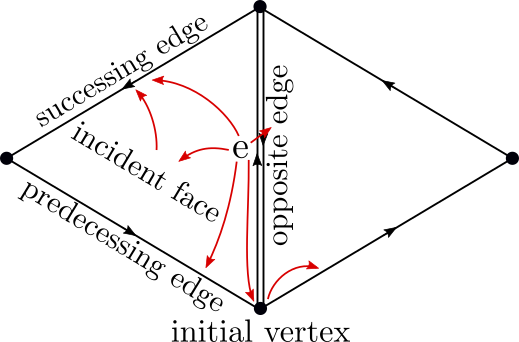
\includegraphics[scale=0.5]{images/img32}}
    \caption[Visualisation of the half-edge data structure]
    {Visualisation of the half-edge data structure.}
    %id obrazku, pomocou ktoreho sa budeme na obrazok odvolavat
    \label{img:32}
\end{figure}

\begin{figure}
    \centerline{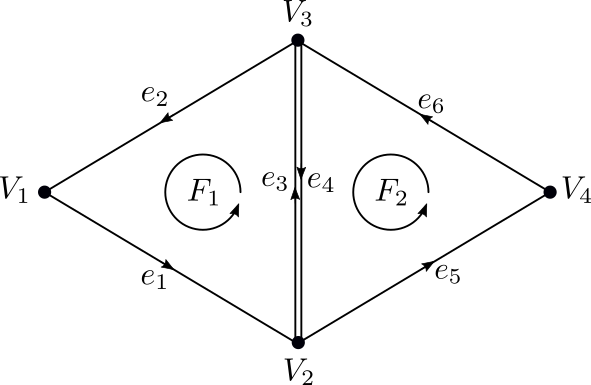
\includegraphics[scale=0.5]{images/img31}}
    \caption[Example of half-edge representation]
    {Example of half-edge representation.}
    %id obrazku, pomocou ktoreho sa budeme na obrazok odvolavat
    \label{img:31}
\end{figure}

\begin{table}[]\centering
    \begin{tabular}{|c|c|c|ccc|}
    \hline
    \hline
    Edge  & Vertex       & Face        & \multicolumn{3}{c|}{Edges}                            \\ \hline
          & Initial      & Incident    & Pred.            & Succ.           & Opposite         \\ \hline\hline
    $e_1$ & $V_1$        & $F_1$       & $e_2$            & $e_3$           &                  \\ \hline
    $e_2$ & $V_3$        & $F_1$       & $e_3$            & $e_1$           &                  \\ \hline
    $e_3$ & $V_2$        & $F_1$       & $e_1$            & $e_2$           & $e_4$            \\ \hline
    $e_4$ & $V_3$        & $F_2$       & $e_6$            & $e_5$           & $e_3$            \\ \hline
    $e_5$ & $V_2$        & $F_2$       & $e_4$            & $e_6$           &                  \\ \hline
    $e_6$ & $V_4$        & $F_2$       & $e_5$            & $e_4$           &                  \\ \hline\hline
    
    \end{tabular}
\caption{Edge table of a half-edge data structure for the Figure \ref{img:31}.}
\label{tab:5}
\end{table}

\begin{table}[]
    \centering
    \begin{tabular}{|c|ccc|c|}
    \hline
    \hline
    Vertex  & \multicolumn{3}{c|}{Coordinates}          & Edge            \\ \hline
          & x            & y            & z           & Outgoing edge   \\ \hline\hline
    $V_1$ & $x_1$        & $y_1$        & $z_1$       & $e_1$           \\ \hline
    $V_2$ & $x_2$        & $y_2$        & $z_2$       & $e_3$           \\ \hline
    $V_3$ & $x_3$        & $y_3$        & $z_3$       & $e_2$           \\ \hline
    $V_4$ & $x_4$        & $y_4$        & $z_4$       & $e_6$           \\ \hline\hline
    \end{tabular}
\caption{Vertex table of a half-edge data structure for the Figure \ref{img:31}.}
\label{tab:6}
\end{table}

\begin{table}[]
    \centering
    \begin{tabular}{|c|c|}
    \hline
    \hline
    Face  & Edge            \\ \hline\hline
    $F_1$ & $e_1$           \\ \hline
    $F_2$ & $e_4$           \\ \hline\hline
    \end{tabular}
\caption{Face table of a half-edge data structure for the Figure \ref{img:31}.}
\label{tab:7}
\end{table}


\subsection{Range tree}
\subsection{Mesh structure}
Triangular mesh consists of vertices, edges and faces. We use the half-edge 
data structure for mesh representation and the range tree for time efficient
search of vertices in three dimensional interval.
The mesh structure used for maintaining and modifying the triangular mesh
consists of:
\begin{itemize}
    \setlength\itemsep{-2mm}
    \item list of vertices,
    \item list of half-edges,
    \item list of faces,
    \item set of active edges,
    \item set of checked edges,
    \item set of bounding edges,
    \item range tree of all vertices.
\end{itemize}
Vertex consists of 
\begin{itemize}
    \setlength\itemsep{-2mm}
    \item three coordinates,
    \item index of itself in the list of vertices,
    \item list of indices to all outgoing edges.
\end{itemize}
Half-edge consists of 
\begin{itemize}
    \setlength\itemsep{-2mm}
    \item six coordinates,
    \item index of itself in the list of half-edges,
    \item index of initial vertex in the list of vertices, 
    \item index of terminal vertex in the list of vertices,
    \item index of opposite edge in the list of half-edges,
    \item index of predecessing edge in the list of half-edges,
    \item index of successing edge in the list of half-edges,
    \item index of incident face in the list of faces.
\end{itemize}
Face consists of
\begin{itemize}
    \setlength\itemsep{-2mm}
    \item nine coordinates,
    \item index of incident half-edge in the list of half-edges.
\end{itemize}

\subsection{Algorithm runtime}
TODO
